\documentclass[parskip=full]{scrartcl}
\usepackage[utf8]{inputenc} % use utf8 file encoding for TeX sources
\usepackage[T1]{fontenc}    % avoid garbled Unicode text in pdf
\usepackage[english]{babel}  % english hyphenation, quotes, etc
\usepackage{hyperref}       % detailed hyperlink/pdf configuration
\hypersetup{                % ‘texdoc hyperref‘ for options
pdftitle={HePICS Design Document},%
bookmarks=true,%
}
\usepackage{graphicx}       % provides commands for including figures
\usepackage{csquotes}       % provides \enquote{} macro for "quotes"
\usepackage{enumitem}


\title{HePICS Design Document}

\begin{document}

\maketitle
\thispagestyle{empty}
\pagebreak





\tableofcontents
\pagebreak





\section {Functionality Description}

In the part of model, the classes realize the management of all the data and logic. They load the path of images and access their features. The results of classification are stored in the type of string to be shown in various forms. The logic of classification is determined by the neural network being used. Its topology defines how different layers interact with each other. With the assistance of all the layers, the forward propagation functionality can be implemented, which is the core of algorithms for image classification with pre-trained model.

The view realizes the user interfaces. The welcome window and the main window, which contains three different sections, guide the user to upload their input files, select available platforms and operating mode, let them control the process and show the prediction results. 

The controller accepts user inputs handled by the components of the views and converts them to the commands. The classifier controls the progress of processing and assigns the scheduler to dispatch work to workers in heterogeneous platforms. In addition, the poller checks the requests from external systems regularly. After receiving the correct request with the image path, the classifier starts the process of classification.

\section {Class Diagram Description}

In this diagram seveal design patterns were used.
In order to decouple  major components and allow parallel development we use the Model-View-Controller as a global architecture.
The class diagram consists of several common patterns to reduce complexity and dependencies between classes.
We use the template Method as pattern for sections to define the skeleton of the algorithm in an operation.
However the results and states are updated using an observer which define a one-to-many dependency between objects.
Different Modes as well as Worker are represented by simple is-relationships.
Another interesting pattern to be used by layers is the strategy-pattern. In this context we define a family of algorithm, encapsulate
each one and make them interchangeable.This approach also lets the algoritm vary independently from the layer that use it.

\pagebreak

\section {Diagrams}

\subsection {Overview Sequence Diagram}

\begin{center}
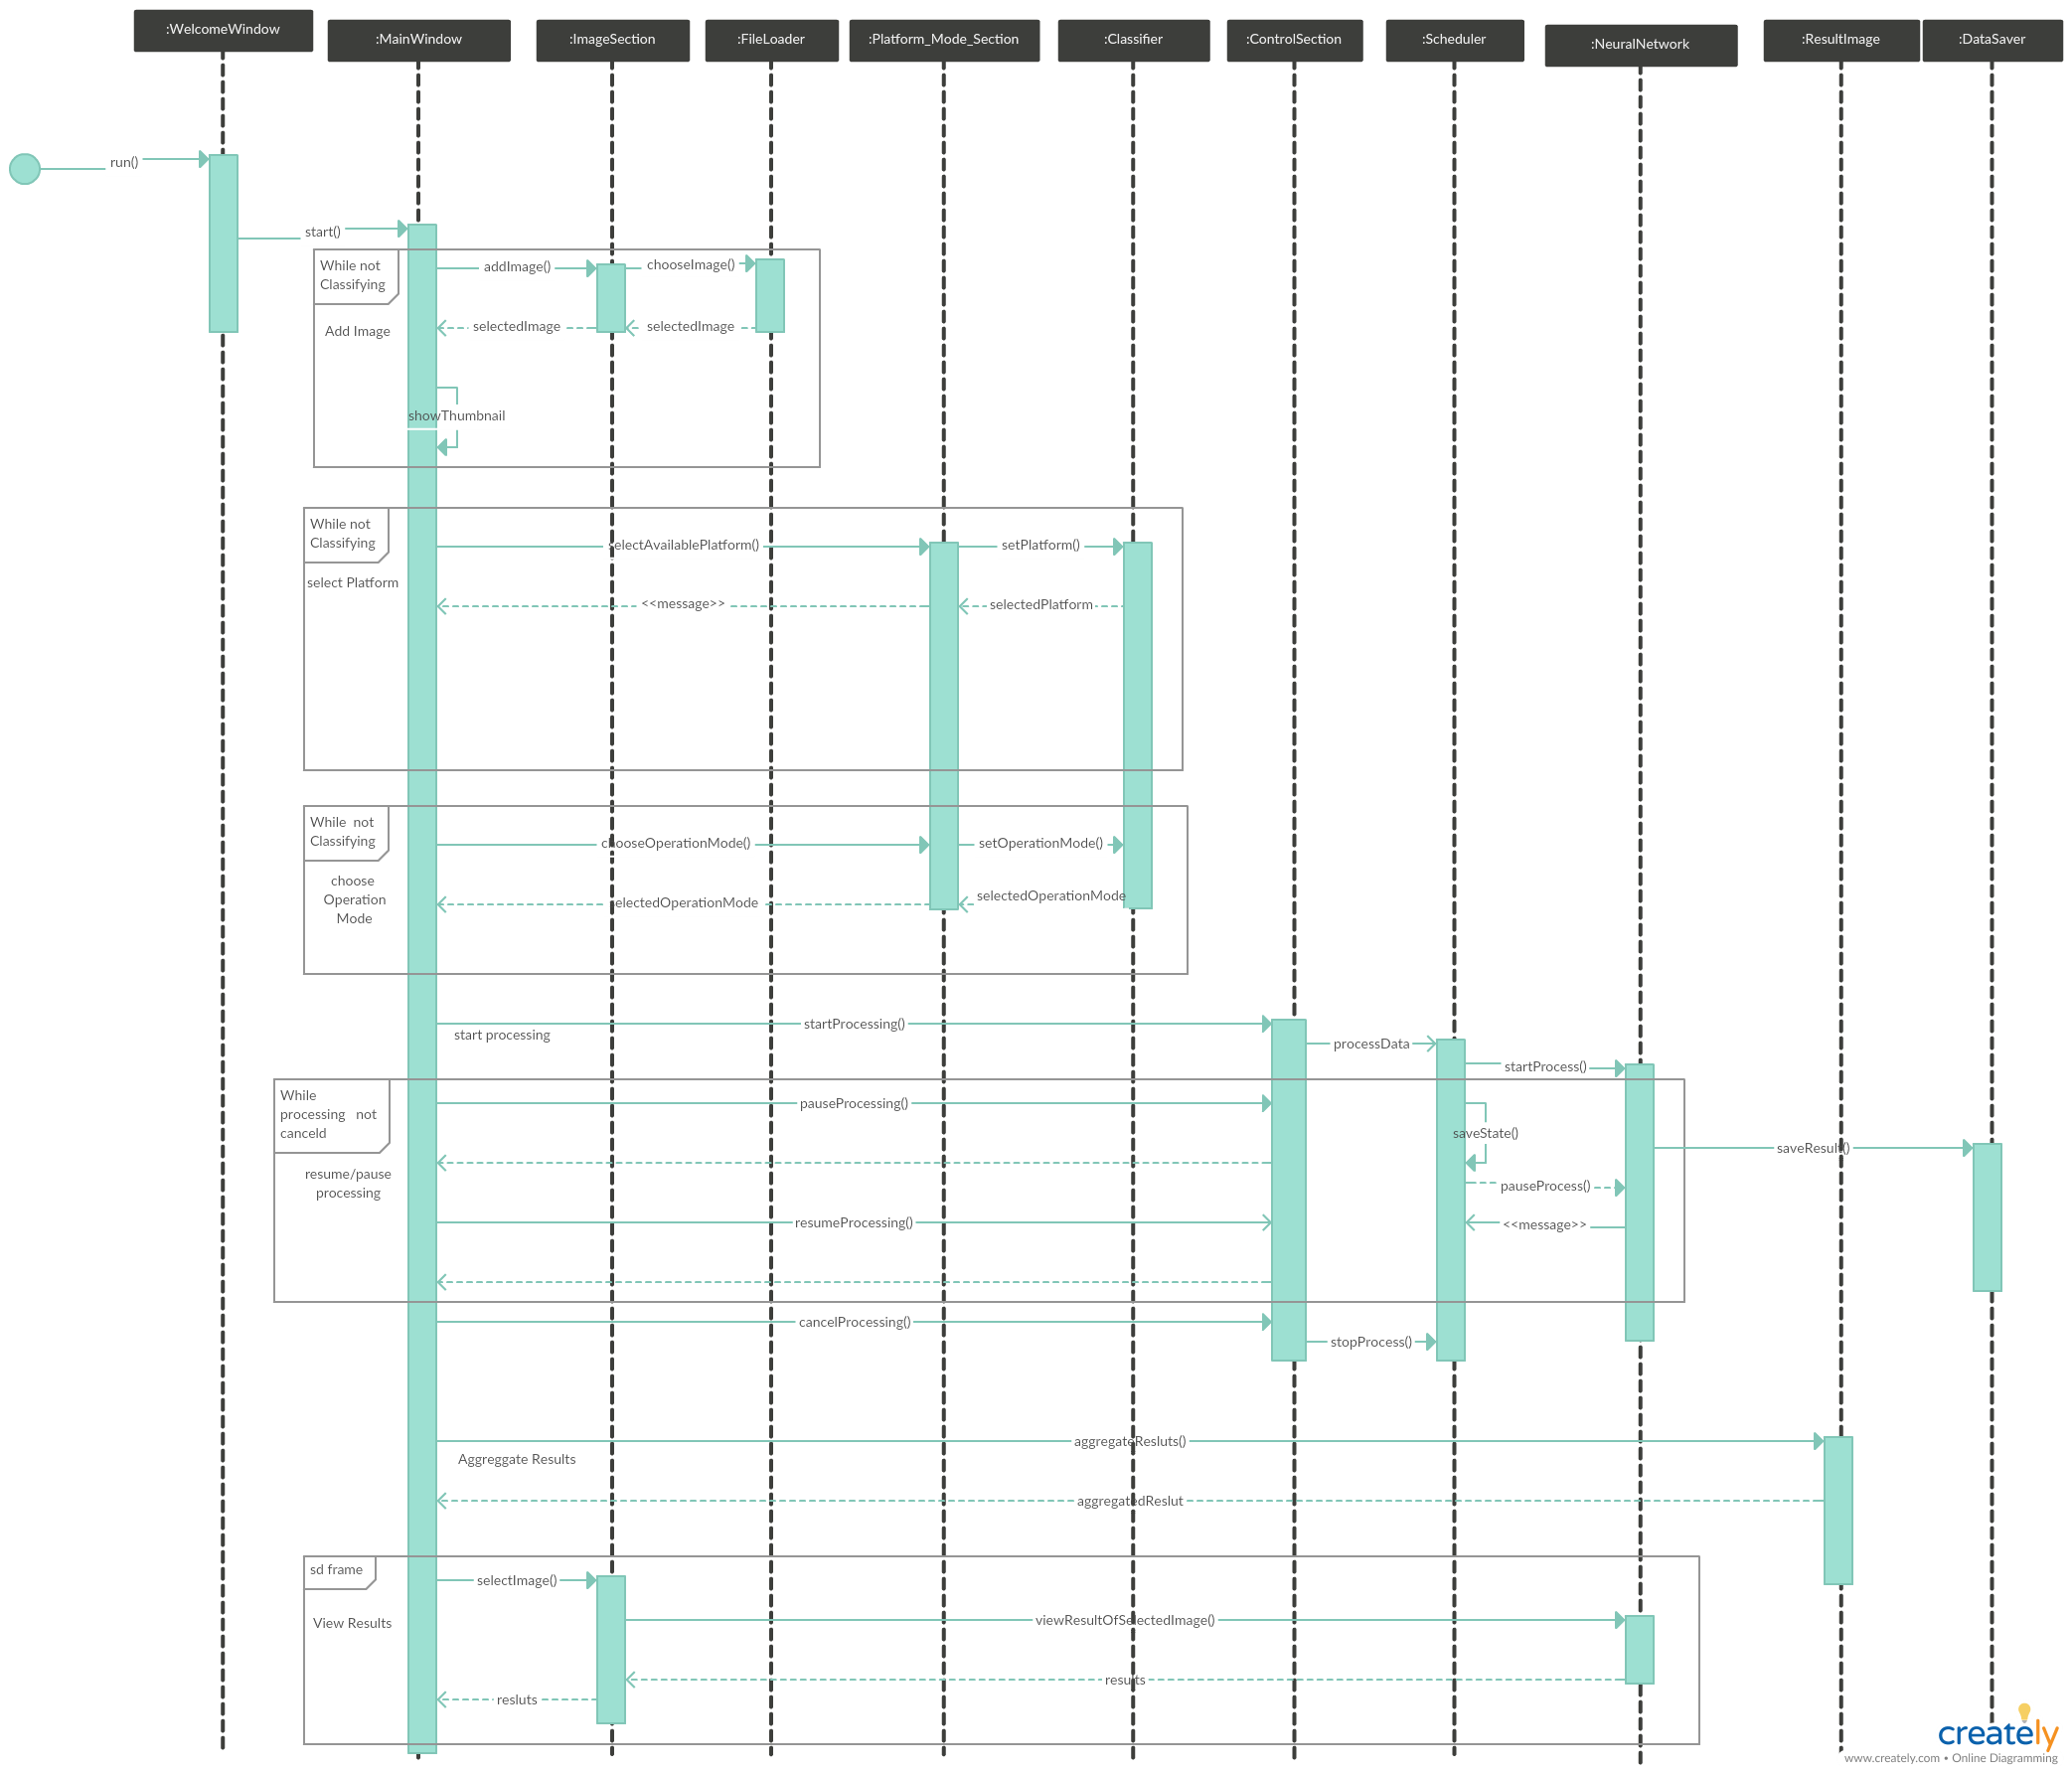
\includegraphics[width=1.0\textwidth]{seq.png}
\end{center}

\pagebreak

\subsection {Select Platforms Sequence Diagram}

\begin{center}
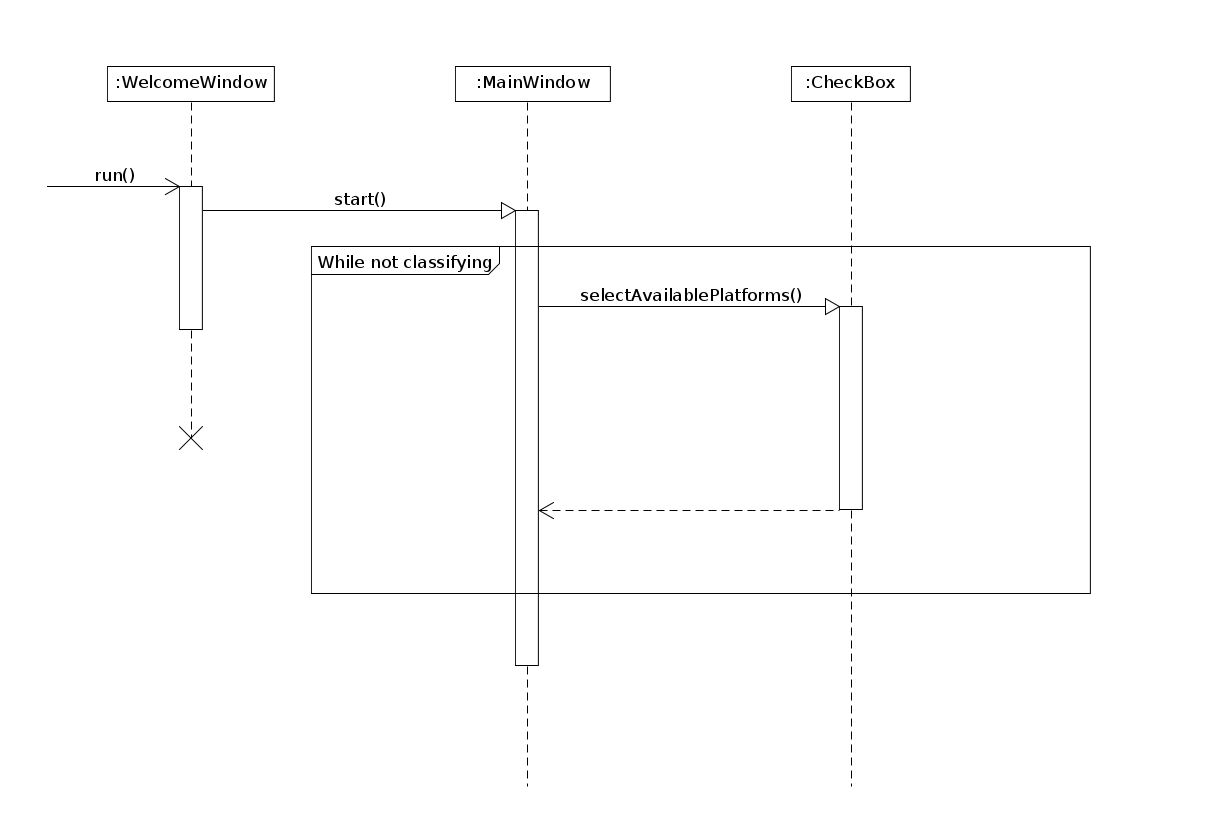
\includegraphics[width=1.0\textwidth]{SelectPlatforms.jpg}
\end{center}

\subsection {Select Image Sequence Diagram}

\begin{center}
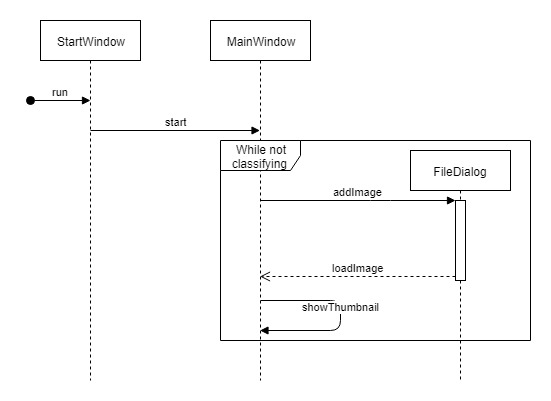
\includegraphics[width=1.0\textwidth]{SelectImageSeqDiag.jpg}
\end{center}

\pagebreak

\subsection {Classification Sequence Diagram}

\begin{center}
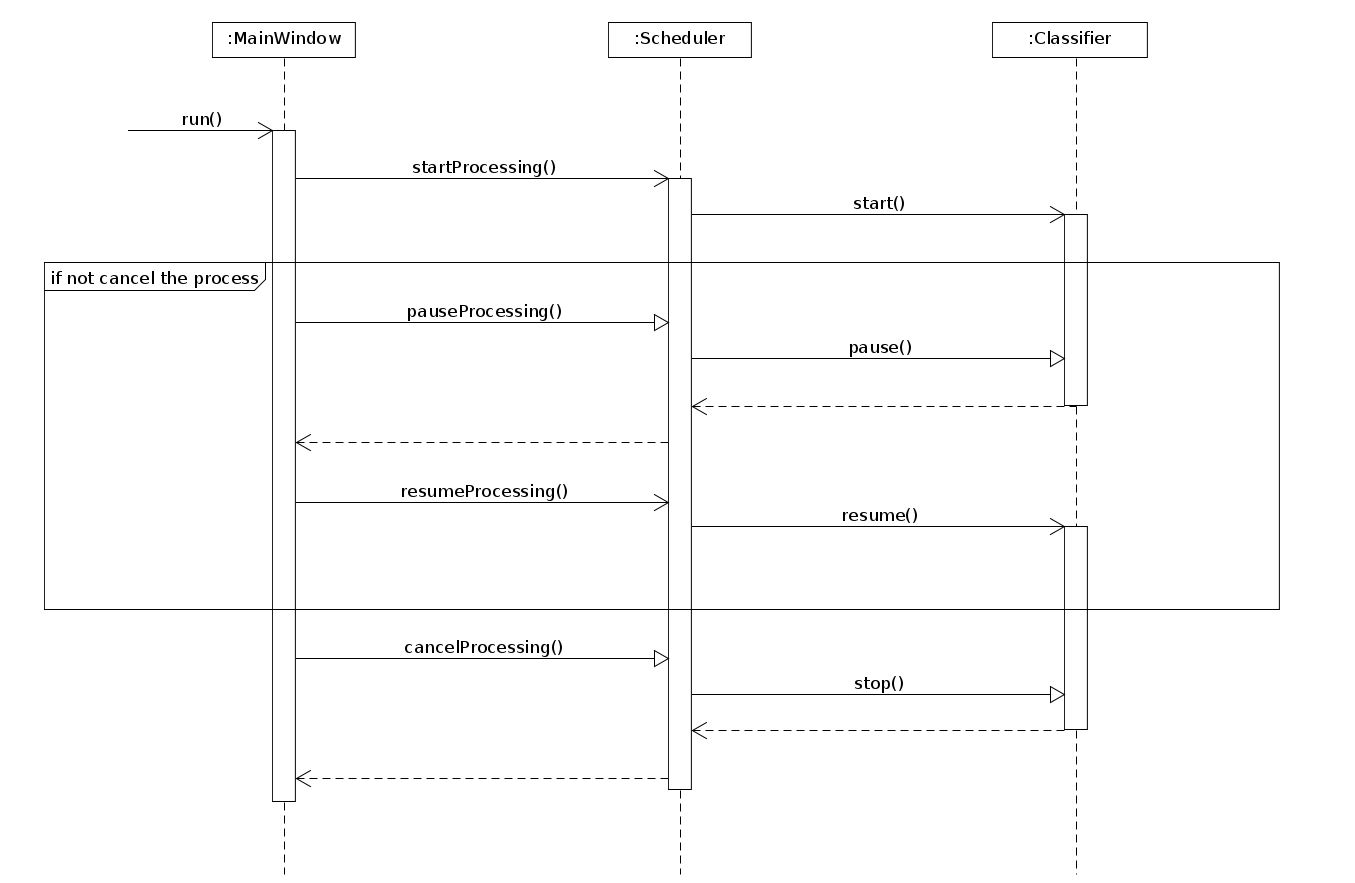
\includegraphics[width=1.0\textwidth]{Classification.jpg}
\end{center}

\pagebreak

\subsection {View Results Sequence Diagram}

\begin{center}
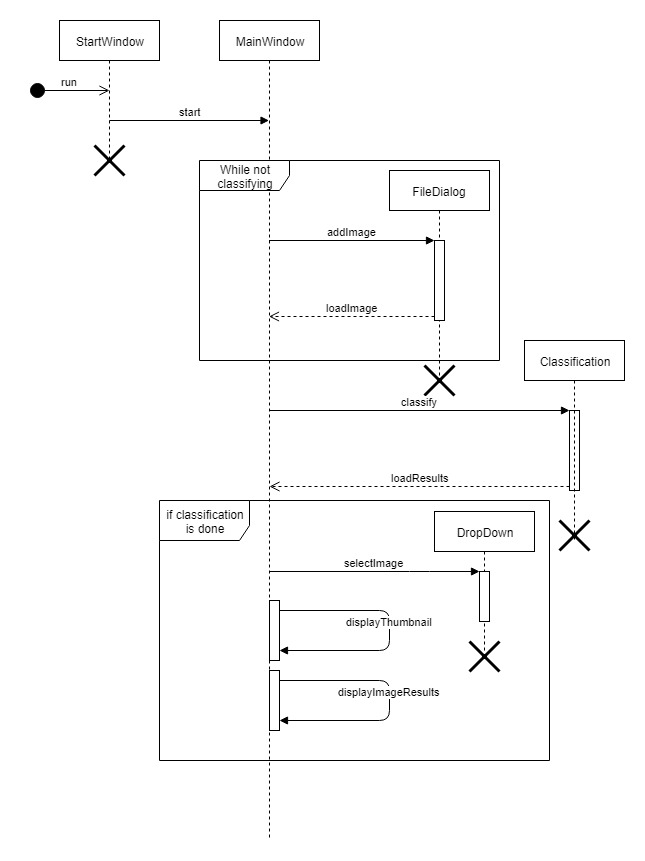
\includegraphics[width=1.0\textwidth]{ViewResults.jpg}
\end{center}

\pagebreak

\subsection {Aggregate Sequence Diagram}

\begin{center}
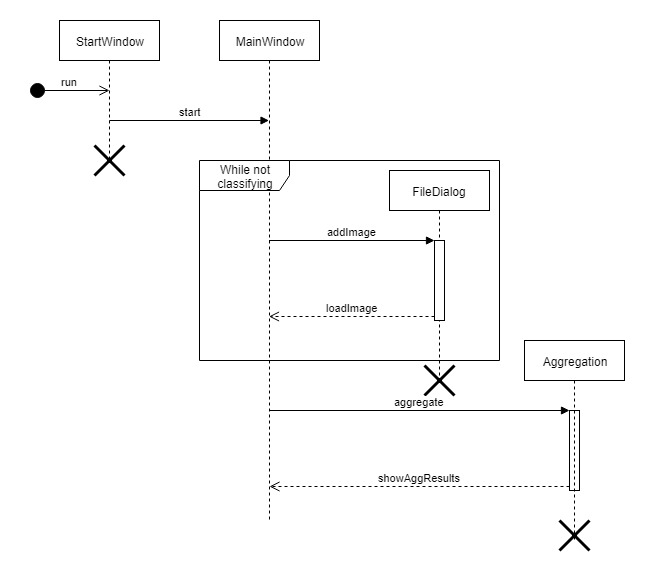
\includegraphics[width=1.0\textwidth]{Aggregate.jpg}
\end{center}

\pagebreak

\subsection {Select Operation Mode Sequence Diagram}

\begin{center}
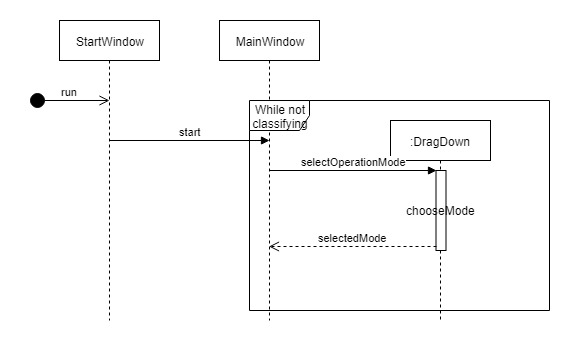
\includegraphics[width=1.0\textwidth]{SelectOperationModeSequenceDiag.jpg}
\end{center}

\pagebreak

\subsection {External Use Sequence Diagram}

\begin{center}
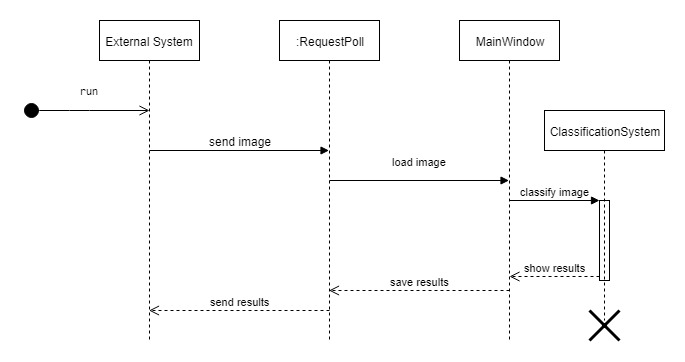
\includegraphics[width=1.0\textwidth]{Untitled Diagram.jpg}
\end{center}

\pagebreak

\subsection {State Diagram}

\begin{center}
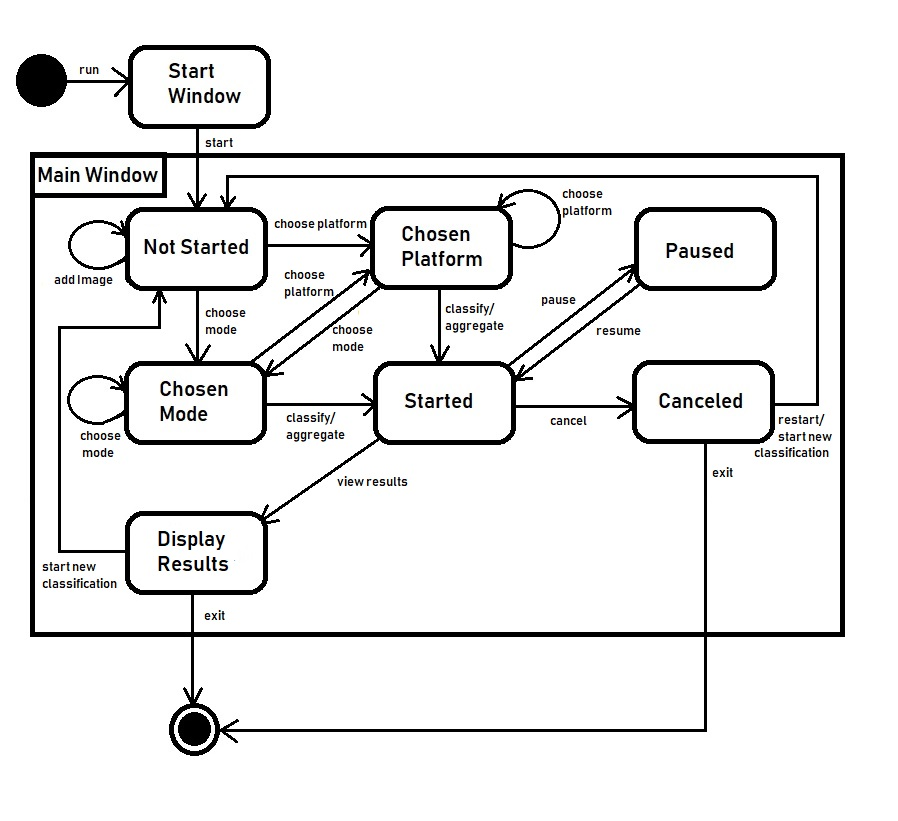
\includegraphics[width=1.0\textwidth]{StateDiag.jpg}
\end{center}

\pagebreak


\end{document}
